\documentclass[11pt,a4paper]{article}

% -----------------------------------------------------------------------------
% CS6868 Research Mini-Project Report
% Safe Memory Reclamation for Lock-Free Data Structures in OCaml 5
% -----------------------------------------------------------------------------

\usepackage[utf8]{inputenc}
\usepackage[T1]{fontenc}
\usepackage[margin=1in]{geometry}
\usepackage{microtype}
\usepackage{lmodern}
\usepackage{amsmath,amssymb}
\usepackage{graphicx}
\usepackage{booktabs}
\usepackage{array}
\usepackage{enumitem}
\usepackage{xcolor}
\usepackage{listings}
\usepackage{pgfplots}
\pgfplotsset{compat=1.18}
\usepackage{hyperref}
\usepackage[capitalise,noabbrev]{cleveref}

\hypersetup{
  colorlinks=true,
  linkcolor=black,
  citecolor=blue!60!black,
  urlcolor=blue!60!black,
}

% --- Listings style -----------------------------------------------------------
\definecolor{codegray}{gray}{0.95}
\definecolor{kw}{RGB}{0,100,170}
\definecolor{cm}{RGB}{100,100,100}
\definecolor{st}{RGB}{170,55,0}
\lstdefinelanguage{ocaml5}{
  morekeywords={let,rec,in,if,then,else,match,with,type,mutable,begin,end,
    fun,function,val,module,struct,sig,open,of,for,to,do,done,while,
    true,false,Some,None,ref,ignore,assert,not},
  sensitive=true,
  morecomment=[s]{(*}{*)},
  morestring=[b]{"},
  literate={->}{{$\to$}}2 {<-}{{$\leftarrow$}}2 {>=}{{$\geq$}}2
           {<=}{{$\leq$}}2 {<>}{{$\neq$}}2 {==}{{$\equiv$}}2,
}
\lstset{
  language=ocaml5,
  basicstyle=\ttfamily\small,
  keywordstyle=\color{kw}\bfseries,
  commentstyle=\color{cm}\itshape,
  stringstyle=\color{st},
  backgroundcolor=\color{codegray},
  frame=single,
  framesep=4pt,
  breaklines=true,
  columns=fullflexible,
  keepspaces=true,
  showstringspaces=false,
  aboveskip=6pt,
  belowskip=4pt,
}

% --- Title block --------------------------------------------------------------
\title{%
  \textbf{CS6868 Research Mini-Project} \\[0.3em]
  \Large Safe Memory Reclamation for Lock-Free Data Structures in OCaml~5%
}
\author{%
  Vishnu Teja Surla \\ \texttt{cs25m050@smail.iitm.ac.in}
  \and
  Ramya Sinigi \\ \texttt{cs25m049@smail.iitm.ac.in}
}
\date{\today}

\begin{document}
\maketitle

% ==============================================================================
\begin{abstract}
% ==============================================================================
We implement and rigorously verify two safe memory reclamation schemes---Hazard
Pointers (HP) and Epoch-Based Reclamation (EBR)---as libraries in OCaml~5,
applying both of them to a lock-free Treiber-stack node pool and EBR to Michael-Scott FIFO
queue. Both schemes eliminate the ABA problem that arises when pre-allocated
nodes are recycled via Compare-And-Swap. We compare them on throughput
(alloc/free cycles per second at 2--8 domains) and memory-boundedness
guarantees. EBR scales positively from 607K to 1\,128K ops/s (2--8 threads),
whereas HP degrades from 470K to 232K due to its $O(R \times N \times K)$ scan.
However, HP bounds unreclaimed garbage to $N \times R$ nodes, while EBR can
delay reclamation indefinitely under stalled threads. Correctness is verified
through five complementary techniques: 24~unit tests, three QCheck-STM suites,
one QCheck-Lin linearizability suite, eight dscheck exhaustive model-checking
tests, and ThreadSanitizer race detection---all reporting zero errors.
\end{abstract}

% ==============================================================================
\section{Goals}
\label{sec:goals}
% ==============================================================================

This project implements two safe memory reclamation schemes---\emph{Hazard
Pointers}~\cite{michael2004hazard} and \emph{Epoch-Based
Reclamation}~\cite{fraser2004practical}---as reusable OCaml~5 libraries.
We apply them to two canonical lock-free data structures: a Treiber-stack
node pool~\cite{treiber1986systems} and then we applied the EBR protection to a 
Michael-Scott FIFO queue~\cite{michael1996simple}, both vulnerable to the ABA
problem~\cite[Ch.~10, \S10.6]{AoMPP} when nodes are recycled.

\medskip
\noindent\textbf{Connection to course topics.}
The project directly exercises concepts from CS6868:
\emph{lock-freedom} via CAS-based stacks and queues (Lectures~7--8),
the \emph{ABA problem} (Lecture~7),
\emph{linearizability} (Lecture~5, verified with QCheck-Lin),
\emph{memory models} and atomic ordering (Lecture~9), and
property-based \emph{verification} (Lectures~10--11).

\medskip
\noindent\textbf{Research question.}
\emph{What is the throughput cost of hazard-pointer scanning vs.\
epoch-based reclamation for protecting a lock-free pool, and how does each
scheme's latency profile differ---given that HP bounds garbage while EBR
can delay reclamation under stalled threads?}

% ==============================================================================
\section{Background}
\label{sec:background}
% ==============================================================================

We assume familiarity with CAS-based lock-free data structures (Treiber
stacks~\cite{treiber1986systems}, Michael-Scott
queues~\cite{michael1996simple}), and the ABA
problem~\cite[Ch.~10, \S10.6]{AoMPP}.  The core question this project
addresses is: \emph{once you remove a node from a lock-free structure, when is
it safe to reclaim or reuse that node?}  A na\"ive answer---``immediately''---is
wrong, because another thread may still hold a stale pointer to the removed
node.  We implement two solutions: Hazard Pointers and Epoch-Based Reclamation.

\subsection{Hazard Pointers (HP)}

Michael~\cite{michael2004hazard} introduced Hazard Pointers as a
\emph{per-access} protection mechanism.  The idea is simple: before you follow
a pointer, you \textbf{announce} it in a globally visible slot so that no other
thread frees the pointed-to node while you are using it.

\paragraph{Data structures.}
Each thread owns $K$ \emph{hazard pointer slots} (typically $K = 1$ or $2$),
stored in a globally readable array.  Each thread also maintains a private
\texttt{retired} list of nodes it has logically removed but cannot yet free.

\paragraph{The load--publish--verify protocol.}
Protecting a pointer requires three steps, shown in pseudocode:

\begin{lstlisting}[caption={HP-protected node access (pseudocode).},
  label={lst:hp}]
(* Step 1: LOAD -- read the shared pointer *)
let node = Atomic.get shared_ptr in

(* Step 2: PUBLISH -- announce it globally *)
hp_slot[my_id] := Some node

(* Step 3: VERIFY -- re-read to detect races *)
if Atomic.get shared_ptr != node then
  (* pointer changed between steps 1 and 2;
     our announcement may protect a freed node.
     Release and retry. *)
  hp_slot[my_id] := None;
  retry ()
else
  (* safe: node cannot be freed while we hold it *)
  use node;
  hp_slot[my_id] := None  (* release when done *)
\end{lstlisting}

Why is the verify step necessary?  Between step~1 (read) and step~2
(publish), another thread could remove and free the node.  Without
re-checking, you would publish a dangling pointer in your HP slot, giving
yourself a false sense of safety while operating on freed memory.

\paragraph{Retiring and scanning.}
When a thread removes a node from the data structure, it does not free it
immediately.  Instead, it \emph{retires} the node---appending it to a
thread-private list along with a cleanup callback.  When the retired list
exceeds a configurable threshold $R$, the thread triggers a \texttt{scan}:

\begin{lstlisting}[caption={HP scan (pseudocode).},label={lst:hpscan}]
let scan () =
  (* Collect all currently protected pointers *)
  let protected = collect_all_hp_slots () in
  List.iter (fun retired_node ->
    if List.mem_phys retired_node protected then
      keep_in_retired_list retired_node
    else
      retired_node.cleanup retired_node  (* safe to free! *)
  ) my_retired_list
\end{lstlisting}

The comparison must use \emph{physical equality} (\texttt{==}, same
object identity) rather than \emph{structural equality} (\texttt{=}, same
value).  Two nodes can hold the same value (e.g., both store~42) but be
different objects; structural equality would incorrectly prevent reclamation.

\paragraph{Complexity and guarantees.}
Each \texttt{scan} collects all $N \times K$ HP slots into a protected set,
then checks each of the $R$ retired nodes against it via linear
search---giving $O(R \times N \times K)$ total work.  The key guarantee is
\textbf{bounded garbage}: at any moment, at most $N \times R$ nodes remain
unreclaimed.  Even if one thread stalls indefinitely, other threads' scans
still reclaim all nodes that the stalled thread is not actively protecting.

\subsection{Epoch-Based Reclamation (EBR)}

Fraser~\cite{fraser2004practical} proposed EBR as a lower-overhead
alternative.  Instead of protecting individual pointers (like HP), EBR
protects \emph{time intervals}: a thread declares ``I am inside a critical
section'' and trusts that nothing retired \emph{before} it entered will be freed
until it exits.

\paragraph{Data structures.}
The system maintains a single \texttt{global\_epoch} counter (starting at~0).
Each thread has two per-thread values: \texttt{local\_epoch} (the epoch it last
observed) and \texttt{active\_count} (the current level of nesting inside the critical section).
Additionally, each thread owns three \emph{limbo buckets}---one per epoch
modulo~3---where retired nodes are collected.

\paragraph{The protocol.}
Critical-section entry, exit, retiring, and epoch advancement work as follows:

\begin{lstlisting}[caption={EBR protocol (pseudocode).},label={lst:ebr}]
let enter () =
  let e = Atomic.get global_epoch in        (* 1. read *)
  Atomic.set my_local_epoch e;              (* 2. publish *)
  Atomic.incr my_active_count;              (* 3. become active *)
  free_limbo_bucket((e + 1) mod 3)          (* 4. free old *)

let exit () =
  Atomic.decr my_active_count

let retire node cleanup =
  let e = Atomic.get global_epoch in
  limbo[e mod 3] := (node, cleanup) :: limbo[e mod 3];
  try_advance_epoch ()

let try_advance_epoch () =
  let e = Atomic.get global_epoch in
  for each thread t do
    if t.active_count > 0 && t.local_epoch < e then
      return  (* someone hasn't caught up yet *)
  done;
  CAS(global_epoch, e, e + 1)  (* all caught up: advance *)
\end{lstlisting}

\paragraph{Why three buckets?}
When the epoch is~$e$, bucket $(e+1) \bmod 3$ corresponds to epoch $e-2$.
Any thread currently active entered at epoch $e-1$ or later, so it cannot hold
references to nodes retired in epoch~$e-2$.  Three buckets give a two-epoch
``grace period'' that guarantees safety.

\paragraph{Why \texttt{active\_count} is an integer.}
If critical sections can nest (e.g., \texttt{dequeue} internally calls
\texttt{enter}/\texttt{exit}), a boolean flag would be cleared by the inner
\texttt{exit}, making the thread appear inactive while the outer function
still holds references.  An integer counter ensures only the outermost
\texttt{exit} (count $\to$ 0) marks the thread as truly inactive.

\paragraph{Why enter ordering matters.}
Steps 1--3 in \texttt{enter} \emph{must} execute in the order shown.  If a
thread increments \texttt{active\_count} \emph{before} setting
\texttt{local\_epoch} and goes to sleep, the epoch advancer sees it as active with a stale epoch (e.g., 0), concludes it hasn't caught up, and \textbf{never advances the
epoch until the sleeping thread wakes up}.

\paragraph{Complexity and guarantees.}
\texttt{enter}/\texttt{exit} are $O(1)$ (a few atomic reads/writes).
\texttt{try\_advance\_epoch} is $O(N)$ (one pass over all threads).  The
trade-off vs.\ HP is that \textbf{garbage is unbounded in the worst case}: if
one thread stalls inside a critical section, the global epoch cannot advance,
and \emph{all} retired nodes from \emph{all} threads remain in limbo
indefinitely.

\subsection{HP vs.\ EBR: summary}

\begin{table}[ht]
\centering\small
\caption{Comparison of HP and EBR at the algorithm level.}
\label{tab:hpvsebr}
\begin{tabular}{@{}lll@{}}
\toprule
& \textbf{Hazard Pointers} & \textbf{EBR} \\
\midrule
Protection granularity & Per-pointer & Per-critical-section \\
Per-access cost & 3 atomics (load, publish, verify) & 1 atomic
  (\texttt{enter}) \\
Scan/advance cost & $O(R \times N \times K)$ & $O(N)$ \\
Worst-case garbage & $N \times R$ (bounded) & Unbounded (stall) \\
Re-entrancy & N.A. (per-pointer) & Requires int counter \\
\bottomrule
\end{tabular}
\end{table}

% ==============================================================================
\section{Tasks Undertaken}
\label{sec:tasks}
% ==============================================================================


\subsection{Implementation}
\label{sec:impl}

The full source is available at
\url{https://github.com/Vishnuteja-Surla/Safe-Memory-Reclamation}.
\Cref{tab:modules} summarises the library modules.

\begin{table}[ht]
\centering\small
\caption{Library modules and their roles.}
\label{tab:modules}
\begin{tabular}{@{}lp{6.5cm}@{}}
\toprule
\textbf{Module} & \textbf{Description} \\
\midrule
\texttt{Lockfree\_pool} & Treiber-stack free list with CAS + exponential
  backoff.  ABA-vulnerable by design. \\
\texttt{Hazard\_pointer} & Global-array HP registry implementing the
  load--publish--verify protocol from \cref{sec:background}. \\
\texttt{Hp\_pool} & Wraps \texttt{Lockfree\_pool} with HP protection;
  exposes \texttt{retired\_count} for test drain loops. \\
\texttt{Ebr} & Three-bucket epoch reclamation implementing the protocol
  from \cref{sec:background}; exposes \texttt{force\_flush}. \\
\texttt{Ebr\_pool} & Wraps \texttt{Lockfree\_pool} with EBR
  enter/exit critical sections. \\
\texttt{Ms\_queue\_ebr} & Michael-Scott queue with internal free list,
  GC fallback, sentinel, helping mechanism, protected using EBR. \\
\bottomrule
\end{tabular}
\end{table}

\subsubsection{Divergence from textbook: global-array registry}
\label{sec:registry}

This is the single most significant departure from the textbook algorithms.
Michael's HP paper~\cite{michael2004hazard} uses a lock-free linked list
of per-thread HP records; Fraser's EBR~\cite{fraser2004practical} assumes
threads can inspect one another's epoch state via shared pointers.
Neither works in OCaml~5: Domain-Local Storage (DLS) is \emph{per-domain
only}---there is no API to read another domain's DLS entry.

Our solution: pre-allocate a \textbf{global flat array} of records, indexed by
domain~ID.  DLS stores only each domain's index into this array:

\begin{lstlisting}
(* HP: slots array readable by all domains *)
type 'a t = {
  slots : 'a option Atomic.t array;
  domain_key : 'a domain_record Domain.DLS.key;
}
(* EBR: records array readable by all domains *)
type 'a t = {
  records : 'a domain_record array;
  domain_key : int Domain.DLS.key;
}
\end{lstlisting}

For HP, each domain owns a contiguous slice
(base = domain\_id $\times$ hp\_per\_domain), giving $O(R \times N \times K)$
scanning with excellent cache locality vs.\ a pointer-chasing linked list.

A second divergence concerns EBR's \textbf{limbo lists}.  The textbook
presents a single global set of limbo buckets shared by all threads; retiring
appends to a shared list, requiring synchronisation.  Our implementation uses
\emph{per-domain} limbo arrays: each domain record contains its own
\texttt{limbo : retired\_node list ref array} (three buckets), so
\texttt{retire} is a simple thread-local list prepend with \emph{zero
contention}.  Reclamation is also local---each domain frees its own limbo
bucket during \texttt{enter}---eliminating cross-domain coordination on the
fast path.

The trade-off for both patterns: \texttt{max\_domains} must be fixed at
creation time (we use 512 after iterating through 128 and
4096---see Bug~2 below).

\subsubsection{OCaml~5 atomic fields and concrete type exposure}

All shared mutable fields use OCaml~5's \texttt{[@atomic]} annotation with the
\texttt{[\%atomic.loc]} PPX, enabling record-level CAS without boxed
\texttt{Atomic.t} cells:

\begin{lstlisting}
type 'a node = {
  mutable value : 'a;
  mutable next : 'a node option; [@atomic]
}
(* CAS directly on a struct field: *)
AL.compare_and_set [%atomic.loc t.top] old_val new_val
\end{lstlisting}

A direct consequence: \texttt{Lockfree\_pool} must \emph{export concrete
record types} in its \texttt{.mli}, breaking encapsulation.
\texttt{Hp\_pool} and \texttt{Ebr\_pool} need
\texttt{[\%atomic.loc t.pool.top]}---impossible with abstract types because the
PPX requires visible field syntax.  Alternatives (internalising HP/EBR logic
in the pool, accessor functions, functors) were rejected for complexity.

\subsubsection{MS~Queue: nominal typing and GC fallback}

The queue maintains its own lock-free free list rather than reusing
\texttt{Lockfree\_pool}: although the node types are structurally identical,
OCaml's \emph{nominal} type system makes them incompatible.
When the free list is exhausted, \texttt{alloc\_node} creates a fresh
GC-allocated node as a fallback, preventing deadlock in producer-heavy
workloads.  \texttt{Ebr\_pool.free} omits \texttt{enter}/\texttt{exit}
(cf.\ \cref{sec:background}) because the caller is relinquishing---not
reading---the node.

\subsubsection{The \texttt{option} boxing discovery}
\label{sec:option-boxing}

Our first ABA demonstration used \lstinline{node option Atomic.t}---and ABA
never triggered.  Each \lstinline{Some} wrapper is a \emph{fresh heap
allocation}, so even when the same node is pushed back, CAS compares different
wrapper addresses and detects the change.  To demonstrate ABA, we bypassed
\lstinline{option} entirely, using direct node pointers with a self-referencing
sentinel node in place of \lstinline{None}.

\subsubsection{Bugs found and fixed}

\paragraph{Bug 1: Domain-registration race (HP and EBR).}
\texttt{fetch\_and\_add} on \texttt{num\_domains} could inflate the count past
\texttt{max\_domains} before the bounds check; a concurrent \texttt{scan}
would access out-of-bounds array slots.
\textbf{Fix:} rollback on failure
(\lstinline{Atomic.fetch_and_add num_domains (-1)}) plus capping the scan
range with \lstinline{min}.

\paragraph{Bug 2: QCheck-Lin domain exhaustion.}
\texttt{Lin\_domain} spawns 2~fresh domains per repetition.  With 300~reps
$\times$ 50~tests, ${\sim}30$K domain creations each permanently consumed an
EBR slot (DLS is not recycled).
\textbf{Fix:} shared instance at module load, \texttt{max\_domains:8192},
reduced test count, and Lin applied only to the MS~Queue.

\paragraph{Bug 3: Weak STM postconditions (EBR pool).}
The original test used \lstinline{true (* accept either *)} for exhausted-pool
allocations, masking memory leaks.  We added \texttt{force\_flush}
(3~enter/retire/exit cycles) to make reclamation synchronous, enabling strict
postconditions: \lstinline{result = (s.free_count > 0)}.

\subsubsection{Testing-support APIs}

\begin{itemize}[nosep]
  \item \texttt{Hp\_pool.retired\_count}: enables drain-until-empty loops;
    improved node recovery from 0/64 to 64/64.
  \item \texttt{Ebr.force\_flush}: makes EBR reclamation synchronous for
    single-domain sequential tests by cycling all 3~limbo buckets.
\end{itemize}

\subsection{Testing and verification}
\label{sec:testing}

We employ five complementary verification techniques, summarised in
\cref{tab:testing}.

\begin{table}[ht]
\centering\small
\caption{Verification techniques and what each catches.}
\label{tab:testing}
\begin{tabular}{@{}llp{4.8cm}@{}}
\toprule
\textbf{Technique} & \textbf{Bug class} & \textbf{How} \\
\midrule
Unit tests (24) & Logic errors, edge cases & Hand-written sequential +
  concurrent scenarios \\
QCheck-STM (3 suites) & Spec.\ violations & Random commands vs.\
  mathematical model \\
QCheck-Lin (1 suite) & Non-linearisable runs & Concurrent interleavings
  on 2 domains \\
dscheck (8 tests) & All-interleaving bugs & Exhaustive atomic schedule
  exploration \\
TSAN (6 suites) & Data races & Compile-time instrumentation \\
\bottomrule
\end{tabular}
\end{table}

\paragraph{ABA stress test.}
Eight domains perform 50\,000 random alloc/free cycles on an 8-node pool.
An atomic ownership array detects double allocation: if
\lstinline{Atomic.exchange ownership.(i) id} returns a non-negative
value, two threads hold the same slot---ABA.
We run two variants: (1)~the \texttt{option}-based \texttt{Lockfree\_pool},
where all three variants (unprotected, HP, EBR) report zero errors because
\lstinline{Some} boxing accidentally prevents ABA
(\cref{sec:option-boxing}); and (2)~a \textbf{direct-pointer} Treiber stack
(sentinel instead of \lstinline{None}, no \lstinline{option} wrapper),
where the unprotected variant shows \textbf{107\,936 ABA errors} while HP
and EBR both report \textbf{zero}.  This definitively proves that HP and EBR
provide genuine algorithmic protection against ABA.

\paragraph{QCheck-STM.}
Each suite defines a simple model (e.g., a bounded counter for the pool, a
list for the queue) and postconditions that must hold after every random
command.  For the EBR pool, we added \texttt{force\_flush} after every
\texttt{Free} to make reclamation synchronous, enabling strict postconditions
(\lstinline{result = (s.free_count > 0)}) instead of the original wildcard
\lstinline{true} that masked memory leaks.

\paragraph{QCheck-Lin (linearizability).}
Applied to the MS~Queue: Lin generates random \texttt{enq}/\texttt{try\_deq}
sequences, runs them concurrently on two domains, and checks that the
observed results match \emph{some} valid sequential ordering.  Pool operations
are unsuitable for Lin because \texttt{free} requires a previously allocated
node---a stateful dependency Lin cannot track.

\paragraph{dscheck (model checking).}
We implement shadow versions of the Treiber stack (4~tests) and MS~Queue
(4~tests) using \texttt{TracedAtomic} so dscheck can intercept atomic
operations.  dscheck then systematically explores every possible interleaving,
checking our assertions (no value loss, no duplicates, FIFO ordering) under
each schedule.

A critical insight: dscheck tests use GC-allocated nodes (fresh addresses per
allocation), making ABA structurally impossible.  The real
\texttt{Lockfree\_pool} recycles pre-allocated nodes---same address
reappears---so HP/EBR are required.  dscheck proves \emph{algorithm
linearizability}; HP/EBR prove \emph{implementation safety}; stress tests prove
\emph{physical correctness}.

\paragraph{TSAN.}
OCaml 5.4.0 with \texttt{ocaml-option-tsan}~\cite{ocamltsan} instruments
every memory access.  All six concurrent test suites report \textbf{zero data
races}, confirming that every shared field is correctly annotated with
\texttt{[@atomic]}.

% ==============================================================================
\section{Evaluation}
\label{sec:evaluation}
% ==============================================================================

\subsection{Experimental setup}

\begin{itemize}[nosep]
  \item \textbf{CPU:} 11th Gen Intel Core i5-11300H @ 3.10\,GHz, 4~cores /
    8~threads.
  \item \textbf{RAM:} 7.6\,GB (WSL2 allocation).
  \item \textbf{OS:} Linux 5.15.167 (WSL2).
  \item \textbf{Compiler:} OCaml 5.4.0 with \texttt{ocaml-option-tsan}.
  \item \textbf{Workload:} 100\,000 alloc+free cycles per domain; 1\,024-node
    pool; 3~runs averaged per configuration.
\end{itemize}

\subsection{Results}

\begin{table}[ht]
\centering
\caption{Throughput (K\,ops/s) for five pool variants at 2--8 threads.}
\label{tab:throughput}
\begin{tabular}{@{}crrrrr@{}}
\toprule
\textbf{Threads} & \textbf{Raw} & \textbf{HP} & \textbf{EBR} &
  \textbf{Mutex} & \textbf{GC} \\
\midrule
2 & 1\,097 & 470 &    607 & 455 & 62\,596 \\
3 &   879 & 464 &    872 & 419 & 53\,003 \\
4 &   733 & 337 & 1\,115 & 311 & 49\,951 \\
5 &   598 & 320 & 1\,347 & 295 & 56\,564 \\
6 &   570 & 282 & 1\,164 & 220 & 42\,824 \\
7 &   519 & 254 & 1\,367 & 212 & 43\,227 \\
8 &   486 & 232 & 1\,128 & 195 & 46\,723 \\
\bottomrule
\end{tabular}
\end{table}

\begin{figure}[ht]
\centering
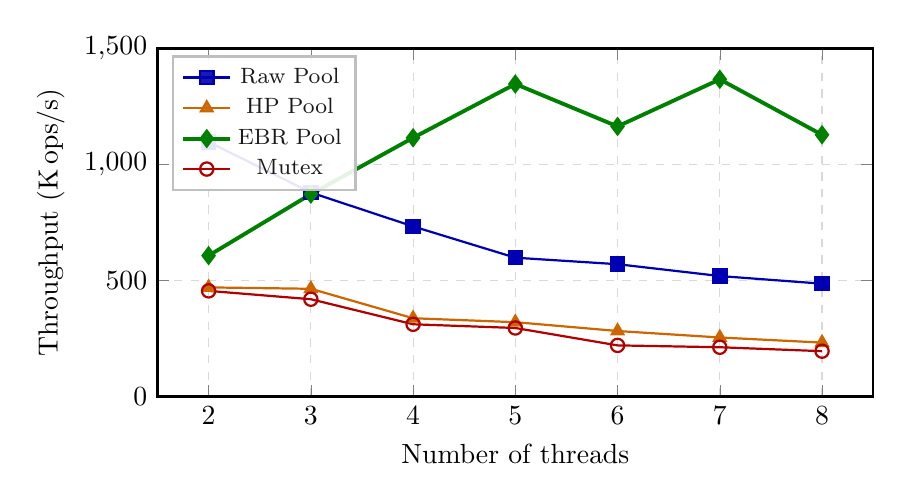
\begin{tikzpicture}
\begin{axis}[
  width=0.88\columnwidth,
  height=6cm,
  ylabel={Throughput (K\,ops/s)},
  xlabel={Number of threads},
  xmin=1.5, xmax=8.5,
  xtick={2,3,4,5,6,7,8},
  ymin=0, ymax=1500,
  legend style={at={(0.02,0.98)}, anchor=north west,
    font=\footnotesize, draw=gray!50, fill=white, fill opacity=0.9},
  grid=major,
  major grid style={dashed, gray!30},
  thick,
  mark options={solid, scale=1.2},
]
\addplot[blue!70!black, mark=square*]
  coordinates {(2,1097) (3,879) (4,733) (5,598) (6,570) (7,519) (8,486)};
\addplot[orange!80!black, mark=triangle*]
  coordinates {(2,470) (3,464) (4,337) (5,320) (6,282) (7,254) (8,232)};
\addplot[green!50!black, mark=diamond*, line width=1.4pt]
  coordinates {(2,607) (3,872) (4,1115) (5,1347) (6,1164) (7,1367) (8,1128)};
\addplot[red!70!black, mark=o]
  coordinates {(2,455) (3,419) (4,311) (5,295) (6,220) (7,212) (8,195)};
\legend{Raw Pool, HP Pool, EBR Pool, Mutex}
\end{axis}
\end{tikzpicture}
\caption{Throughput scaling for the four pool-based variants (GC-only
  allocation omitted; it achieves 43--63M\,ops/s).  EBR scales
  positively with thread count; HP, Raw, and Mutex all degrade.}
\label{fig:throughput}
\end{figure}

\begin{table}[ht]
\centering
\caption{Verification results: all suites pass with zero errors.}
\label{tab:verification}
\begin{tabular}{@{}lrl@{}}
\toprule
\textbf{Suite} & \textbf{Tests} & \textbf{Result} \\
\midrule
Unit tests (6 suites) & 24 & All pass \\
QCheck-STM (HP pool, EBR pool, MS queue) & 2\,100 cases & All pass \\
QCheck-Lin (MS queue) & 300 reps & Linearisable \\
dscheck (pool + MS queue) & 8 & All interleavings pass \\
TSAN (6 suites) & --- & 0 races \\
ABA stress (HP/EBR) & 400\,000 ops & 0 double-allocs \\
\bottomrule
\end{tabular}
\end{table}

\subsection{Discussion}

\paragraph{Finding 1: OCaml's GC dominates throughput.}
GC-only allocation achieves 43--63M ops/s---two orders of magnitude faster
than any pool scheme.  OCaml~5's minor-heap allocator is essentially a
pointer bump; the GC handles deallocation concurrently.  Explicit pools are
justified only for deterministic latency or bounded memory, not raw throughput.

\paragraph{Finding 2: EBR scales positively; HP degrades.}
As shown in \cref{fig:throughput}, EBR scales from 607K (2T) to 1\,128K
(8T)---throughput nearly doubles.  This occurs because EBR's
\texttt{enter}/\texttt{exit} serialises domains just enough to reduce CAS
contention on the pool's \texttt{top} pointer.  HP, by contrast, drops from
470K to 232K ($2.0\times$ degradation) because each \texttt{scan} reads all
$N \times K$ slots ($R$ retired nodes $\times$ $N \times K$ protected entries).
At 8~threads, EBR delivers $4.9\times$ the throughput
of HP.

\paragraph{Finding 3: Mutex collapses under contention.}
Mutex throughput drops from 455K (2T) to 195K (8T)---a $2.3\times$ collapse
due to the classic lock-convoy effect.

\paragraph{Finding 4: Raw pool is fastest at low thread counts, but unsafe.}
The unprotected pool achieves the highest throughput at 2~threads (1\,097K)
but degrades to 486K at 8~threads and is vulnerable to ABA errors under
recycling.

\paragraph{Finding 5: EBR is the recommended safe scheme.}
EBR is the only variant whose throughput \emph{increases} with thread count,
making it the clear winner for OCaml~5 workloads with predictable domain
lifetimes.  HP is preferable only when stall-resilient memory bounds are
required.

% ==============================================================================
\section{Reflection on the Use of LLMs}
\label{sec:llm}
% ==============================================================================

\paragraph{Tools and models used.}
We used \textbf{Claude Opus 4.6 (Antigravity)} as an AI coding assistant in
pair-programming mode.  It had full workspace access: reading/writing files,
running terminal commands (with approval), and executing tests.  It was used
for code generation, debugging, explaining algorithms, writing test harnesses,
and drafting documentation.

\paragraph{What worked well.}
The LLM excelled at \textbf{boilerplate generation and API scaffolding}:
\texttt{.mli} interface files, \texttt{dune} build configurations, and test
harnesses were produced quickly and accurately.  It performed well at
\textbf{translating algorithmic descriptions into OCaml code}---given
Michael's HP paper~\cite{michael2004hazard}, it produced a working
implementation with the correct global-array registry pattern on the first
attempt.  The iterative workflow (implement $\to$ test $\to$ diagnose $\to$
fix) was highly productive.

\paragraph{What did not work.}
The LLM initially struggled with \textbf{OCaml~5-specific features} like
\texttt{[@atomic]} field annotations and the \texttt{[\%atomic.loc]} PPX.
Early attempts used \texttt{Atomic.t} record fields instead of
\texttt{[@atomic] mutable} fields, requiring significant rework.  It also
produced an EBR pool STM test with \textbf{overly permissive postconditions}
(\lstinline{true (* accept either *)}) that masked potential bugs---a flaw
caught only during manual audit.  Lesson: LLM-generated tests require the same
scrutiny as LLM-generated implementations.

\paragraph{What was surprising.}
The most surprising discovery was OCaml's \textbf{\texttt{option} boxing
preventing ABA} in GC-allocated stacks.  The LLM initially generated ABA
demonstrations using \lstinline{'a node option Atomic.t}, which never
triggered ABA because each \lstinline{Some} wrapper is a fresh heap allocation.
The LLM eventually provided the correct diagnosis---address identity
vs.\ structural equality in \lstinline{compare_and_set}---after several failed
attempts.

\paragraph{What was difficult.}
The hardest challenges involved \textbf{interactions between multiple concurrent
systems}: EBR epoch advancement, DLS lifecycle, and QCheck's domain-spawning
strategy.  The QCheck-Lin domain-exhaustion bug required understanding three
components: DLS key initialisation, \texttt{Lin\_domain}'s internal spawning,
and EBR slot allocation.  The \texttt{max\_domains} sizing problem
($128 \to 4096 \to 512$) required iterative experimentation.

\paragraph{Your overall assessment.}
The LLM was an effective \textbf{accelerator}, reducing implementation time by
an estimated 60--70\%.  However, every audit-discovered flaw was found through
manual review.  The most productive workflow was:
\emph{LLM generates, human audits, LLM fixes, human verifies}.

% ==============================================================================
\section{Conclusions}
\label{sec:conclusions}
% ==============================================================================

\paragraph{Answering the research question.}
HP imposes a $2.1$--$2.3\times$ throughput penalty vs.\ the unprotected pool
(1\,097K$\to$470K at 2T, 486K$\to$232K at 8T).  EBR, remarkably,
\textbf{scales positively}: 607K at 2T rising to 1\,128K at 8T,
\emph{surpassing} the raw pool at $\geq$4~threads.
The gap between EBR and HP widens from $1.3\times$ at 2T to $4.9\times$ at 8T
because HP's \texttt{scan} is $O(R \times N \times K)$ while EBR's
\texttt{enter}/\texttt{exit} is $O(1)$.

Regarding latency profiles: \textbf{HP has bounded garbage}---at most
$N \times R$ nodes are unreclaimed ($N$~domains, $R$~retire threshold).
\textbf{EBR can delay reclamation} if a domain stalls in a critical section,
preventing epoch advancement and leaving \emph{all} retired nodes in limbo.
Our \texttt{test\_multi\_domain\_protection} verifies this directly.

\paragraph{Limitations.}
(1)~\texttt{max\_domains} is fixed at creation time; dynamic expansion is not
implemented.
(2)~dscheck tests the algorithm (GC-allocated nodes) rather than the production
code (\texttt{[@atomic]} fields); the GC-vs-recycling divergence means ABA is
not tested in dscheck.
(3)~Verification is empirical, not a formal proof of linearisability.
(4)~\texttt{Obj.magic ()} is used for placeholder values in pool creation and
\texttt{force\_flush}.

\paragraph{Future work.}
Lock-free dynamic expansion of the HP/EBR registry; an HP-based MS~Queue for
direct HP-vs-EBR queue comparison; formal verification with the Iris separation
logic framework; tail-latency (p99/p999) benchmarking to reveal GC pause effects.

% ==============================================================================
\section*{Contributions}
\label{sec:contributions}
% ==============================================================================

\begin{center}
\begin{tabular}{@{}lcp{5.5cm}@{}}
\toprule
\textbf{Member} & \textbf{\%} & \textbf{Main responsibilities} \\
\midrule
Vishnu Surla (CS25M050) & 30\% & HP, Lockfree Pool, HP Pool implementation \\
Ramya Sinigi (CS25M049) & 30\% & EBR, EBR Pool, MS Queue EBR implementation \\
Joint (both members) & 40\% & All testing (unit, QCheck-STM, QCheck-Lin,
  dscheck, TSAN, stress), benchmarking, documentation, code audits \\
\midrule
\textbf{Total} & \textbf{100\%} & \\
\bottomrule
\end{tabular}
\end{center}

% ==============================================================================
\bibliographystyle{plainurl}
\bibliography{references}
% ==============================================================================

\end{document}
